\documentclass[../../../main]{subfiles}
\begin{document}

\section{結果・課題}

\subsection{課題1}

ある一つの粒子について、原点を適当に定め座標を5秒ごとに記録した結果を表\ref{tab:position}に示す。
なお、座標の有効数字はソフトウェア上では\SI{1}{\nano\meter}のオーダーまで計測できていたが、光学顕微鏡の分解能はおおよそ光の波長程度であり、\SI{10}{\nano\meter}のオーダーを四捨五入し、\SI{100}{\nano\meter}のオーダーにした。
また、表\ref{tab:position}の$x_m$と$y_m$は、\SI{10}{\micro\meter}ごとに線が切られたマイクロメーターをソフトウェア上で5回計測した結果が表\ref{tab:micrometer}で、その平均が\SI{10.04}{\micro\meter}であったから、$x_m = x \times \dfrac{10}{10.04}$と$y_m = y \times \dfrac{10}{10.04}$として校正した値である。
$\Delta x_m$、$\Delta y_m$はそれぞれ$x_m$、$y_m$の差分である。
この $\Delta x_m$、$\Delta y_m$についてヒストグラムを作成すると、図\ref{fig:delta-x-y-histogram}のようになる。

\begin{longtable} {c}
    \caption{\SI{10}{\micro\meter}のソフトウェア上での計測結果} \label{tab:micrometer} \\
    \hline 距離 $d$ /\SI{}{\micro\meter}                                   \\ \hline
    \endfirsthead

    \hline
    \endlastfoot
    9.9                                                                  \\
    9.9                                                                  \\
    10                                                                   \\
    10.2                                                                 \\
    10.2                                                                 \\
\end{longtable}

\newpage
\begin{longtable}{ccccccc}
    \caption{粒子の座標} \label{tab:position}                                                                                                                                                                               \\
    \hline 時間 $T$ /\SI{}{\sec} & $x$ /\SI{}{\micro\meter} & $y$ /\SI{}{\micro\meter} & $x_m$ /\SI{}{\micro\meter} & $y_m$ /\SI{}{\micro\meter} & $\Delta x_m$ /\SI{}{\micro\meter} & $\Delta y$ /\SI{}{\micro\meter}   \\ \hline
    \endfirsthead
    \hline 時間 $T$ /\SI{}{\sec} & $x$ /\SI{}{\micro\meter} & $y$ /\SI{}{\micro\meter} & $x_m$ /\SI{}{\micro\meter} & $y_m$ /\SI{}{\micro\meter} & $\Delta x$ /\SI{}{\micro\meter}   & $\Delta y_m$ /\SI{}{\micro\meter} \\ \hline
    \endhead
    \hline \multicolumn{7}{r}{次のページへ続く。}                                                                                                                                                                               \\ \hline
    \endfoot
    \hline
    \endlastfoot
    0                          & 71.2                     & 60.8                     & 70.9                       & 60.6                       & -                                 & -                                 \\
    5                          & 72.0                     & 59.1                     & 71.7                       & 58.8                       & 0.8                               & -1.8                              \\
    10                         & 69.7                     & 58.5                     & 69.4                       & 58.3                       & -2.3                              & -0.6                              \\
    15                         & 68.7                     & 56.6                     & 68.4                       & 56.4                       & -1.0                              & -1.9                              \\
    20                         & 69.1                     & 54.3                     & 68.8                       & 54.1                       & 0.4                               & -2.3                              \\
    25                         & 67.2                     & 53.9                     & 66.9                       & 53.7                       & -1.9                              & -0.4                              \\
    30                         & 64.0                     & 53.5                     & 63.7                       & 53.2                       & -3.2                              & -0.5                              \\
    35                         & 64.7                     & 52.8                     & 64.4                       & 52.6                       & 0.7                               & -0.7                              \\
    40                         & 63.7                     & 53.4                     & 63.4                       & 53.1                       & -1.0                              & 0.6                               \\
    45                         & 63.2                     & 53.4                     & 62.9                       & 53.1                       & -0.5                              & 0.0                               \\
    50                         & 61.4                     & 53.3                     & 61.2                       & 53.1                       & -1.8                              & -0.1                              \\
    55                         & 60.1                     & 51.5                     & 59.9                       & 51.3                       & -1.3                              & -1.8                              \\
    60                         & 59.2                     & 51.4                     & 59.0                       & 51.2                       & -0.9                              & -0.1                              \\
    65                         & 56.1                     & 49.3                     & 55.9                       & 49.1                       & -3.1                              & -2.0                              \\
    70                         & 53.6                     & 49.6                     & 53.4                       & 49.4                       & -2.5                              & 0.3                               \\
    75                         & 52.8                     & 48.1                     & 52.6                       & 47.9                       & -0.8                              & -1.5                              \\
    80                         & 53.5                     & 47.0                     & 53.3                       & 46.8                       & 0.7                               & -1.1                              \\
    85                         & 53.1                     & 46.4                     & 52.9                       & 46.3                       & -0.4                              & -0.6                              \\
    90                         & 53.8                     & 44.2                     & 53.6                       & 44.0                       & 0.7                               & -2.2                              \\
    95                         & 51.7                     & 41.3                     & 51.5                       & 41.1                       & -2.1                              & -2.9                              \\
    100                        & 50.4                     & 42.2                     & 50.2                       & 42.1                       & -1.3                              & 0.9                               \\
    105                        & 47.8                     & 40.7                     & 47.6                       & 40.5                       & -2.6                              & -1.6                              \\
    110                        & 46.3                     & 36.9                     & 46.1                       & 36.8                       & -1.5                              & -3.7                              \\
    115                        & 42.0                     & 35.7                     & 41.8                       & 35.6                       & -4.3                              & -1.2                              \\
    120                        & 40.1                     & 35.9                     & 39.9                       & 35.7                       & -1.9                              & 0.2                               \\
    125                        & 36.4                     & 35.6                     & 36.3                       & 35.5                       & -3.7                              & -0.3                              \\
    130                        & 34.5                     & 34.7                     & 34.4                       & 34.5                       & -1.9                              & -0.9                              \\
    135                        & 31.9                     & 32.7                     & 31.8                       & 32.6                       & -2.6                              & -2.0                              \\
    140                        & 32.4                     & 30.7                     & 32.3                       & 30.5                       & 0.5                               & -2.0                              \\
    145                        & 31.9                     & 31.0                     & 31.8                       & 30.9                       & -0.5                              & 0.4                               \\
    150                        & 31.0                     & 29.8                     & 30.9                       & 29.7                       & -0.9                              & -1.2                              \\
    155                        & 30.2                     & 29.1                     & 30.1                       & 28.9                       & -0.8                              & -0.7                              \\
    160                        & 29.3                     & 27.0                     & 29.2                       & 26.9                       & -0.9                              & -2.0                              \\
    165                        & 24.6                     & 24.7                     & 24.5                       & 24.6                       & -4.7                              & -2.3                              \\
    170                        & 23.9                     & 22.1                     & 23.8                       & 22.1                       & -0.7                              & -2.5                              \\
    175                        & 22.0                     & 21.4                     & 21.9                       & 21.3                       & -1.9                              & -0.7                              \\
    180                        & 20.4                     & 21.0                     & 20.3                       & 20.9                       & -1.6                              & -0.4                              \\
    185                        & 18.4                     & 21.3                     & 18.3                       & 21.2                       & -2.0                              & 0.3                               \\
    190                        & 20.1                     & 19.5                     & 20.0                       & 19.5                       & 1.7                               & -1.8                              \\
    195                        & 20.6                     & 16.8                     & 20.5                       & 16.8                       & 0.5                               & -2.7                              \\
    200                        & 18.6                     & 14.9                     & 18.5                       & 14.8                       & -2.0                              & -2.0                              \\
    205                        & 14.7                     & 12.9                     & 14.6                       & 12.8                       & -3.9                              & -2.0                              \\
    210                        & 14.5                     & 13.8                     & 14.4                       & 13.8                       & -0.2                              & 0.9                               \\
    215                        & 13.2                     & 11.3                     & 13.1                       & 11.3                       & -1.3                              & -2.5                              \\
    220                        & 10.3                     & 9.2                      & 10.3                       & 9.1                        & -2.9                              & -2.1                              \\
    225                        & 8.2                      & 6.8                      & 8.2                        & 6.8                        & -2.1                              & -2.3                              \\
    230                        & 8.2                      & 7.8                      & 8.2                        & 7.7                        & 0.0                               & 0.9                               \\
    235                        & 7.3                      & 6.4                      & 7.3                        & 6.3                        & -0.9                              & -1.4                              \\
    240                        & 4.3                      & 5.0                      & 4.3                        & 4.9                        & -3.0                              & -1.4                              \\
    245                        & 2.0                      & 5.1                      & 2.0                        & 5.1                        & -2.3                              & 0.2                               \\
    250                        & 2.0                      & 3.7                      & 2.0                        & 3.7                        & 0.0                               & -1.4                              \\
\end{longtable}


\newpage
\begin{figure}[htbp]
    \centering
    \begin{minipage}[b]{0.45\linewidth}
        \centering
        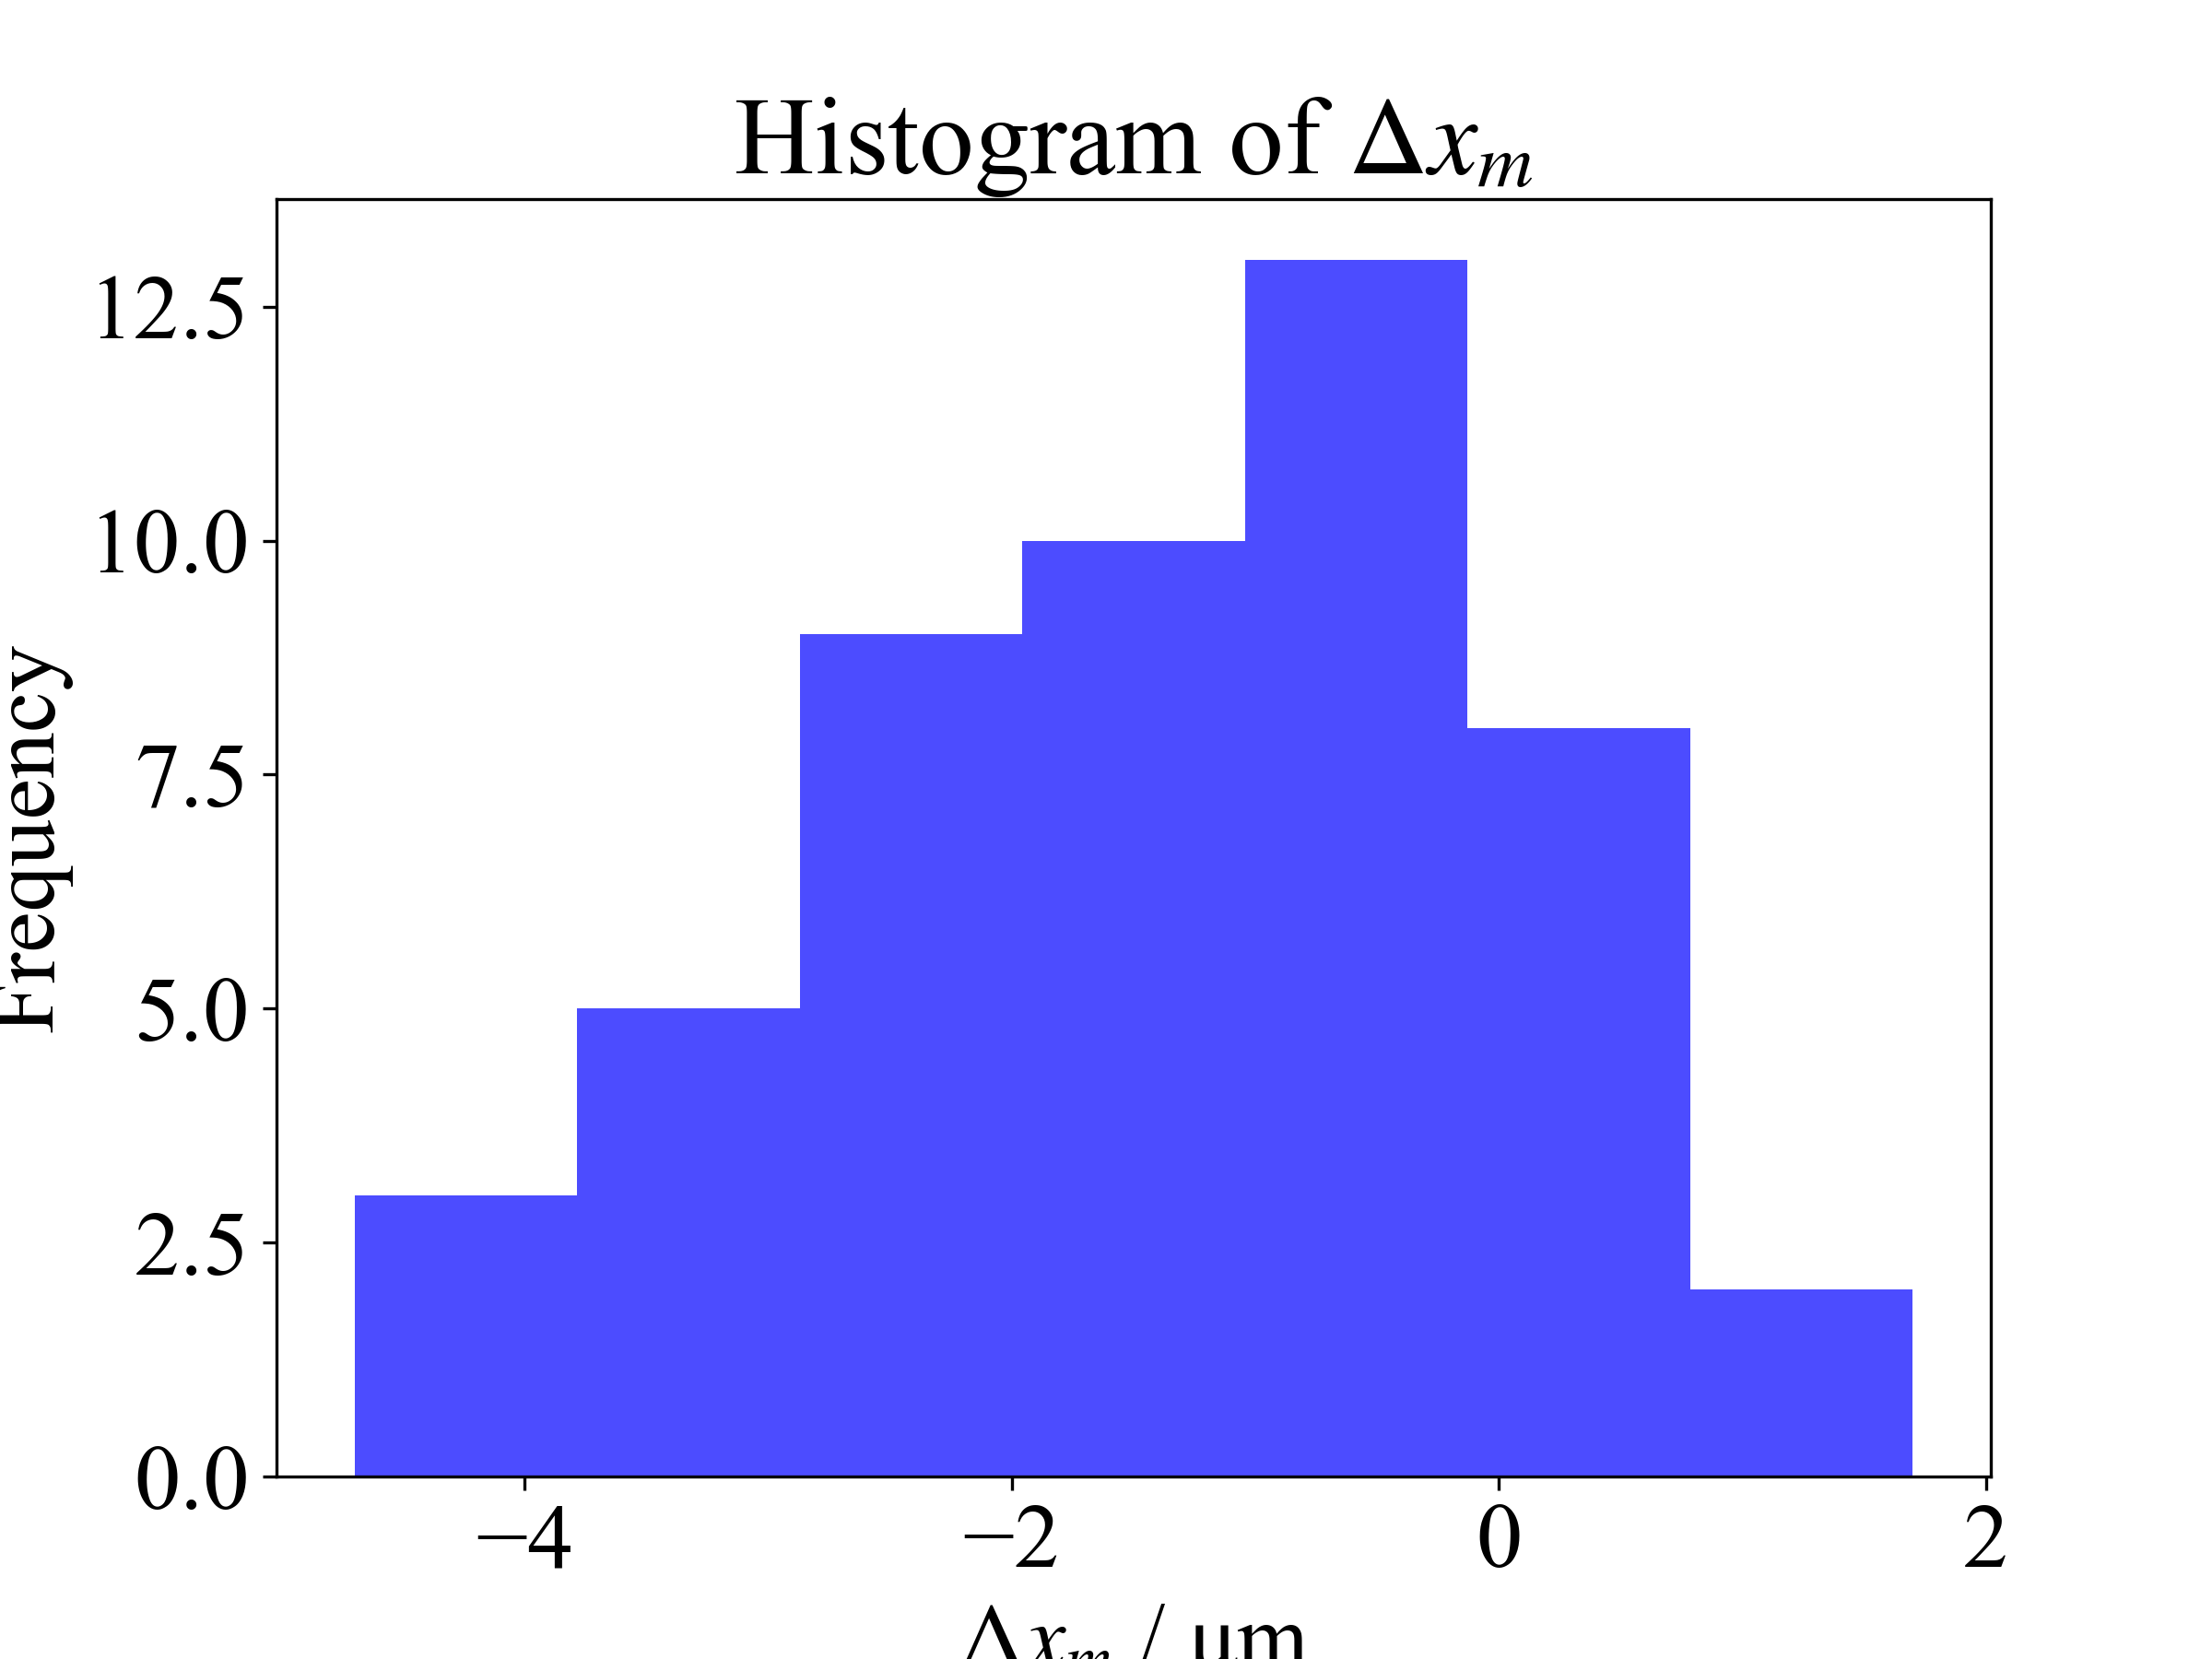
\includegraphics[keepaspectratio, width=\linewidth]{src/figures/delta-x-y-histogram/delta-x-histogram.png}
        \subcaption{$\Delta x_m$}
    \end{minipage}
    \begin{minipage}[b]{0.45\linewidth}
        \centering
        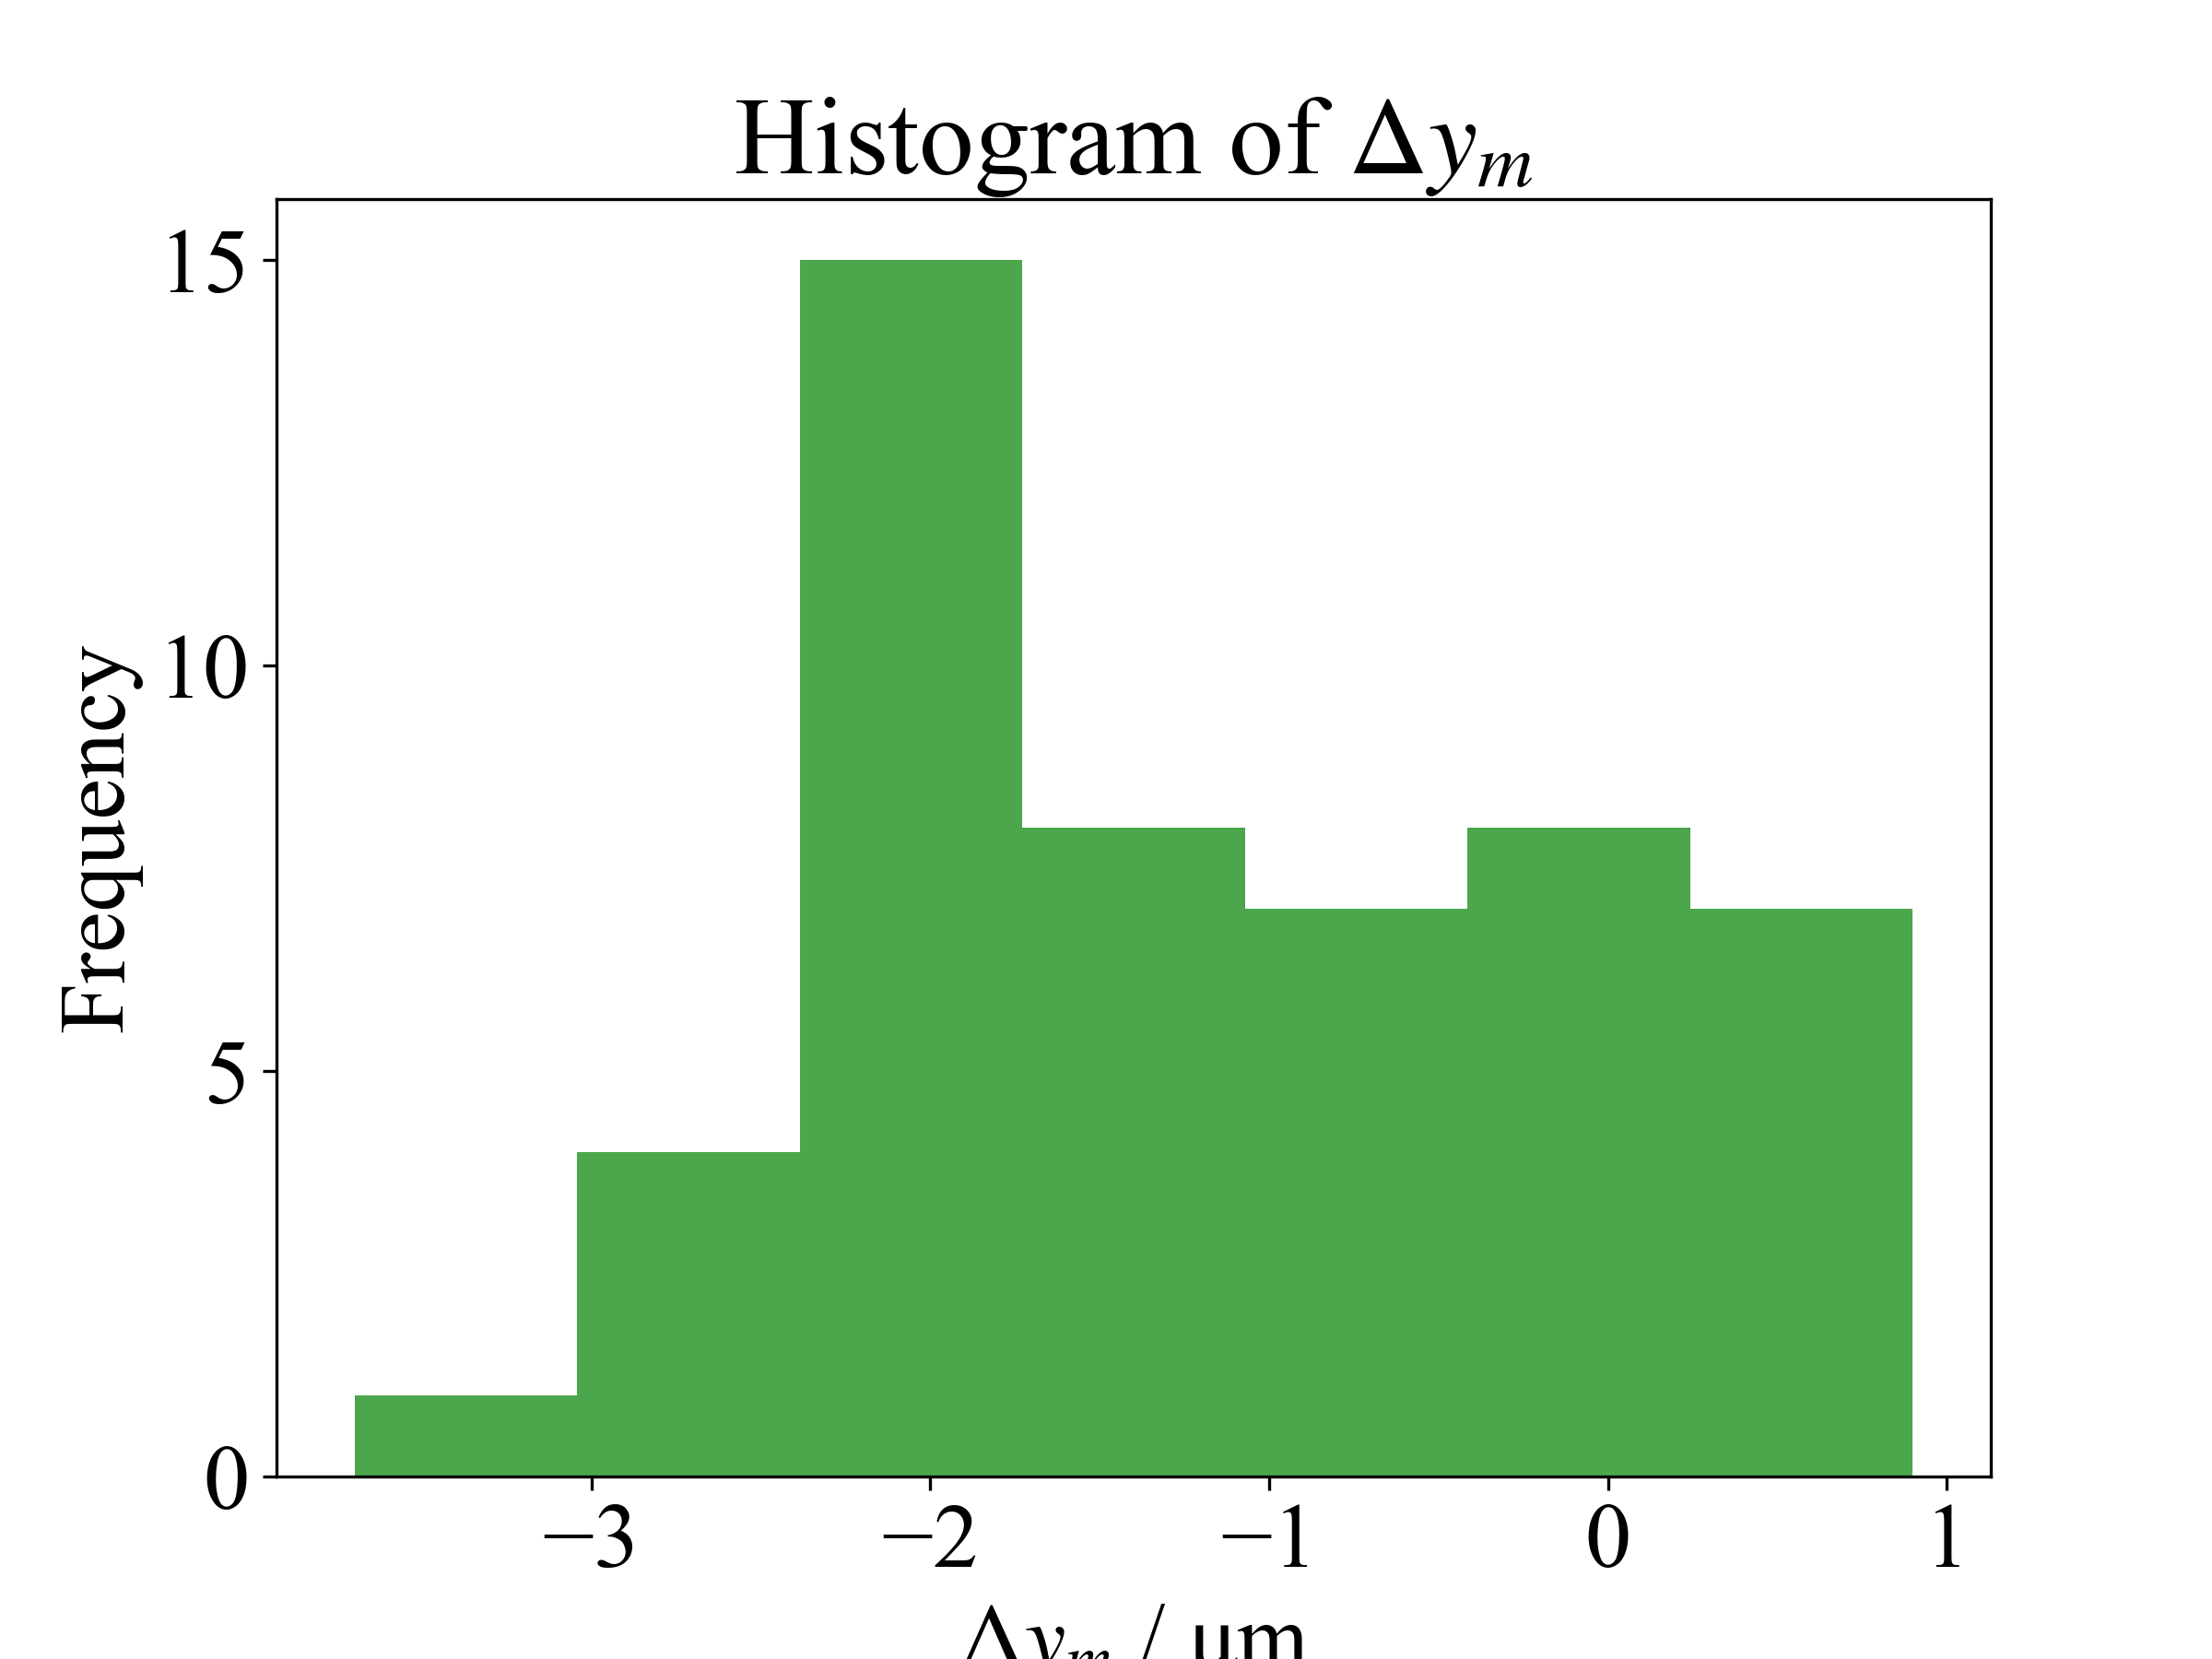
\includegraphics[width=\linewidth]{src/figures/delta-x-y-histogram/delta-y-histogram.png}
        \subcaption{$\Delta y_m$}
    \end{minipage}
    \caption{$\Delta x_m$と$\Delta y_m$のヒストグラム} \label{fig:delta-x-y-histogram}
\end{figure}


\clearpage
\subsection{課題2}

表\ref{tab:position}をもとに、
$x_m$の分散$\ev{(x_m-\ev{x_m})^2}=\ev{(\Delta x_m)^2}$、
$y_m$の分散$\ev{(y_m-\ev{y_m})^2}=\ev{(\Delta y_m)^2}$、
移動量$\sqrt{(\Delta x_m)^2 + (\Delta y_m)^2}$の分散、$\ev{(\Delta x_m)^2 + (\Delta y_m)^2}$を求めると、
次の表\ref{tab:position-variance}のようになる。

\begin{longtable}{ccc}
    \caption{粒子の座標の分散} \label{tab:position-variance}                                                                                                                                     \\
    \hline $\ev{(\Delta x_m)^2}$ /\SI{}{\micro\meter\squared} & $\ev{(\Delta y_m)^2}$ /\SI{}{\micro\meter\squared} & $\ev{(\Delta x_m)^2 + (\Delta y_m)^2}$ /\SI{}{\micro\meter\squared} \\ \hline
    \endfirsthead
    \hline $\ev{(\Delta x_m)^2}$ /\SI{}{\micro\meter\squared} & $\ev{(\Delta y_m)^2}$ /\SI{}{\micro\meter\squared} & $\ev{(\Delta x_m)^2 + (\Delta y_m)^2}$ /\SI{}{\micro\meter\squared} \\ \hline
    \endhead
    \hline
    \endfoot

    3.86                                                      & 2.52                                               & 6.39                                                                \\
\end{longtable}


ブラウン運動の力学的な考察から、
\begin{equation}\label{eq:brownian-motion}
    \ev{(\Delta x_m)^2} = \dfrac{kT}{3\pi a \eta} t = \dfrac{RT}{3 \pi a \eta N_A} t
\end{equation}
が成り立つ。
ここで、$k$はボルツマン定数、$T$は温度、$a$は粒子の半径、$\eta$は溶媒の粘度、$R$は気体定数、$N_A$はアボガドロ数である。
理科年表\cite{rika-nenpyo}によると、
室温は$T=\SI{299.35}{\kelvin}$、
粒子半径は$a=\SI{1.50}{\micro\meter}$、
気体定数は$R=\SI{8.3144598}{\joule\per\kelvin\per\mole}$
である。
$\eta$は水の粘度であるが、次の表\ref{tab:water-viscosity}のようになる。
指数関数でフィッティングすると、
次の\ref{eq:water-viscosity}式のようになりこれをもとに室温\SI{26.6}{\celsius}で水の粘度は\SI{0.84965}{\milli\pascal\second}であると考えられる。
\begin{equation}\label{eq:water-viscosity}
    \eta = 1.7599 \times \exp(-0.027793T) \si{\milli\pascal\second}
\end{equation}

\begin{longtable}{cc}
    \caption{水の温度と粘度の関係} \label{tab:water-viscosity}               \\
    \hline 温度 / \SI{}{\celsius} & 粘度 / \SI{}{\milli\pascal\second} \\ \hline
    \endfirsthead
    \hline 温度 / \SI{}{\celsius} & 粘度 / \SI{}{\milli\pascal\second} \\ \hline
    \endhead
    \hline
    \endfoot
    0                           & 1.7906                           \\
    5                           & 1.5185                           \\
    10                          & 1.3064                           \\
    15                          & 1.1378                           \\
    20                          & 1.0016                           \\
    25                          & 0.8899                           \\
    30                          & 0.7970                           \\
\end{longtable}


以上を踏まえて、アボガドロ定数、ボルツマン定数を計算すると以下のようになる。
\begin{align}
    k_{x_m} & = \dfrac{\ev{(\Delta x_m)^2} \cdot 3 \pi a \eta}{tT}                                                                                                            \nonumber          \\
            & = \dfrac{\SI{3.86}{\micro\meter\squared} \cdot 3 \pi \cdot \SI{1.50}{\micro\meter} \cdot \SI{0.84965}{\milli\pascal\second}}{\SI{5}{\second} \cdot \SI{299.35}{\kelvin}} \nonumber \\
            & = \SI{3.10E-23}{\joule\per\kelvin}                                                                                                                                                 \\
    k_{y_m} & = \SI{2.03E-23}{\joule\per\kelvin}
\end{align}
\begin{align}
    N_{x_m} & = \dfrac{R}{k_{x_m}} = \dfrac{\SI{8.3144598}{\joule\per\kelvin\per\mole}}{\SI{3.10E-23}{\joule\per\kelvin}} \nonumber \\
            & = \SI{2.68E23}{\per\mole}                                                                                             \\
    N_{y_m} & = \SI{4.09E23}{\per\mole}
\end{align}

なお、文献値は$N_A=\SI{6.02214076E23}{\per\mole}$、$k=\SI{1.38064852E-23}{\joule\per\kelvin}$である。

\clearpage
\subsection{課題3}
\ref{subsec:report-2}で求めた$k_{x_m}$、$k_{y_m}$の誤差を定量的に考察する。

$N_A$は、$N_A=R/k$であるから、$k$を用いて考える。
$k_{x_m}$、$k_{y_m}$それぞれ相対誤差は次のようになる。
\begin{align}
    \delta k_{x_m} & = \dfrac{\left| k_{x_m} - k \right|}{ k_{x_m} } \nonumber \\
                   & = \SI{55.5}{\percent}                                     \\
    \delta k_{y_m} & = \SI{31.9}{\percent}
\end{align}

まず、$k$と$T$の関係を考える。
$\eta$は表\ref{tab:water-viscosity}のように温度依存性があり、$k$も\ref{eq:brownian-motion}式から温度を含む。
$T$は溶液の温度であるが、実際に計測したのは室温である。
したがって、室温と溶液の温度の差が誤差の一因として考えられる。
$\eta$と、$k$の$T$依存性は次の\ref{fig:k-n-relation}のようになる

\begin{figure}[htbp]
    \centering
    \begin{minipage}[b]{0.45\linewidth}
        \centering
        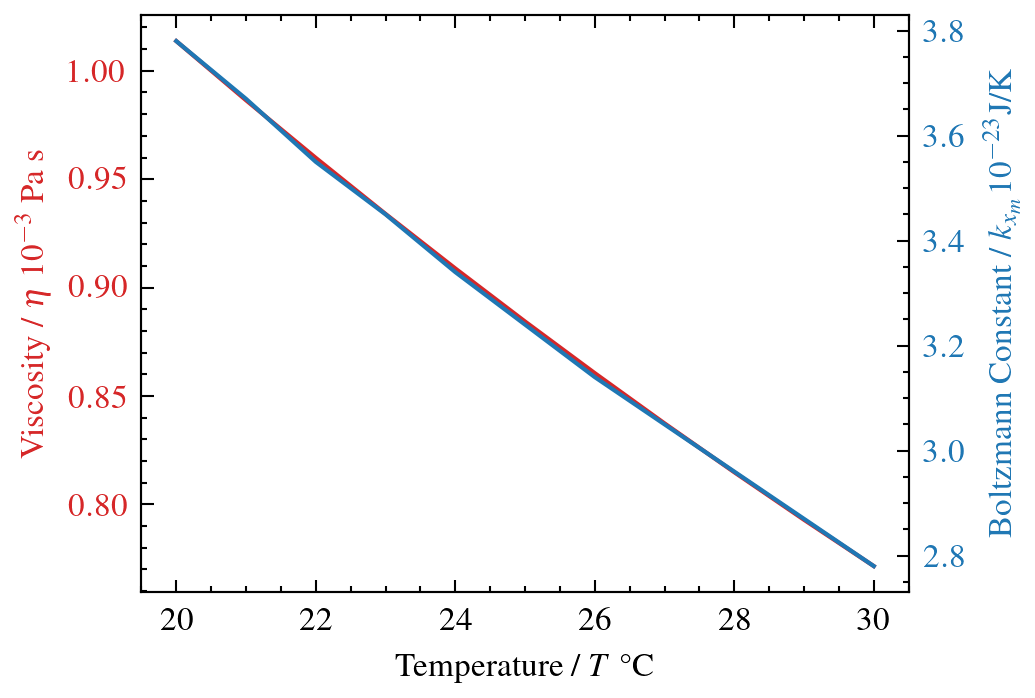
\includegraphics[keepaspectratio, width=\linewidth]{src/figures/k-n-relation/k-x-n-relation.png}
        \subcaption{$k_{x_m}$}
    \end{minipage}
    \begin{minipage}[b]{0.45\linewidth}
        \centering
        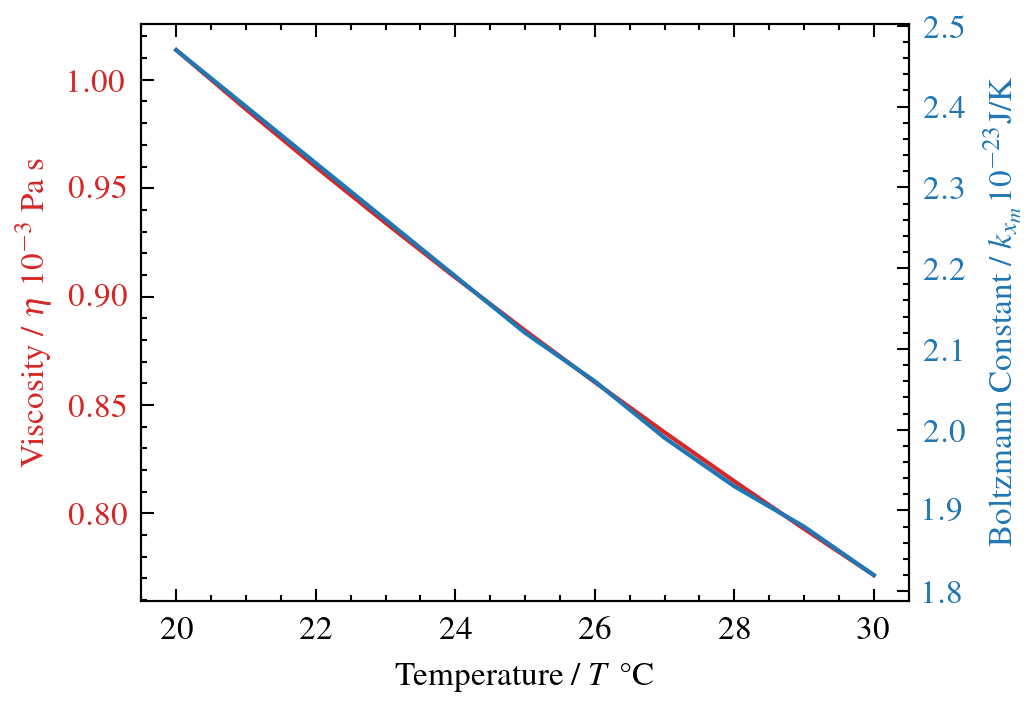
\includegraphics[width=\linewidth]{src/figures/k-n-relation/k-y-n-relation.png}
        \subcaption{$k_{y_m}$}
    \end{minipage}
    \caption{$k$と$\eta$の$T$依存性} \label{fig:k-n-relation}
\end{figure}


実際に計測された室温は\SI{26.6}{\celsius}で、
この周辺で$\eta$はほぼ線形で、同様に$k$も線形であると考えられる。
グラフから温度が\SI{1}{\celsius}異なると、
$\eta$はおよそ\SI{0.025}{\milli\pascal\second}変化している。
$k_{m_x}$は、\SI{0.07E-23}{\joule\per\kelvin}、
$k_{m_y}$は、\SI{0.06E-23}{\joule\per\kelvin}変化している。
したがって、十分長い時間溶液は放置され室温に近い温度になっていたとすれば、
温度の誤差は高々\SI{1}{\celsius}であるとして、
$k_{x_m}$、$k_{y_m}$の誤差はそれぞれ
$\SI{0.07E-23}{\joule\per\kelvin}$、$\SI{0.06E-23}{\joule\per\kelvin}$であると考えられる。

次に、$k$の$\ev{(\Delta x)^2}$依存性を考える。
式\ref{eq:brownian-motion}からわかる様に、$k$は$\ev{(\Delta x)^2}$に比例する。
これを図示すると、次の図\ref{fig:k-x-relation}のようになる。
このグラフから、$k$の理論値に対する$\ev{(\Delta x)^2}$は\SI{1.64}{\micro\meter\squared}であると計算できる。

$k_{x_m}$の相対誤差は\SI{57.5}{\percent}で2.35倍、
$k_{y_m}$の相対誤差は\SI{34.9}{\percent}で1.54倍であると計算できる。
よって本実験では、粒子のブラウン運動が理論値に比べて大きくランダムに運動していたとわかる。


\begin{figure}
    \centering
    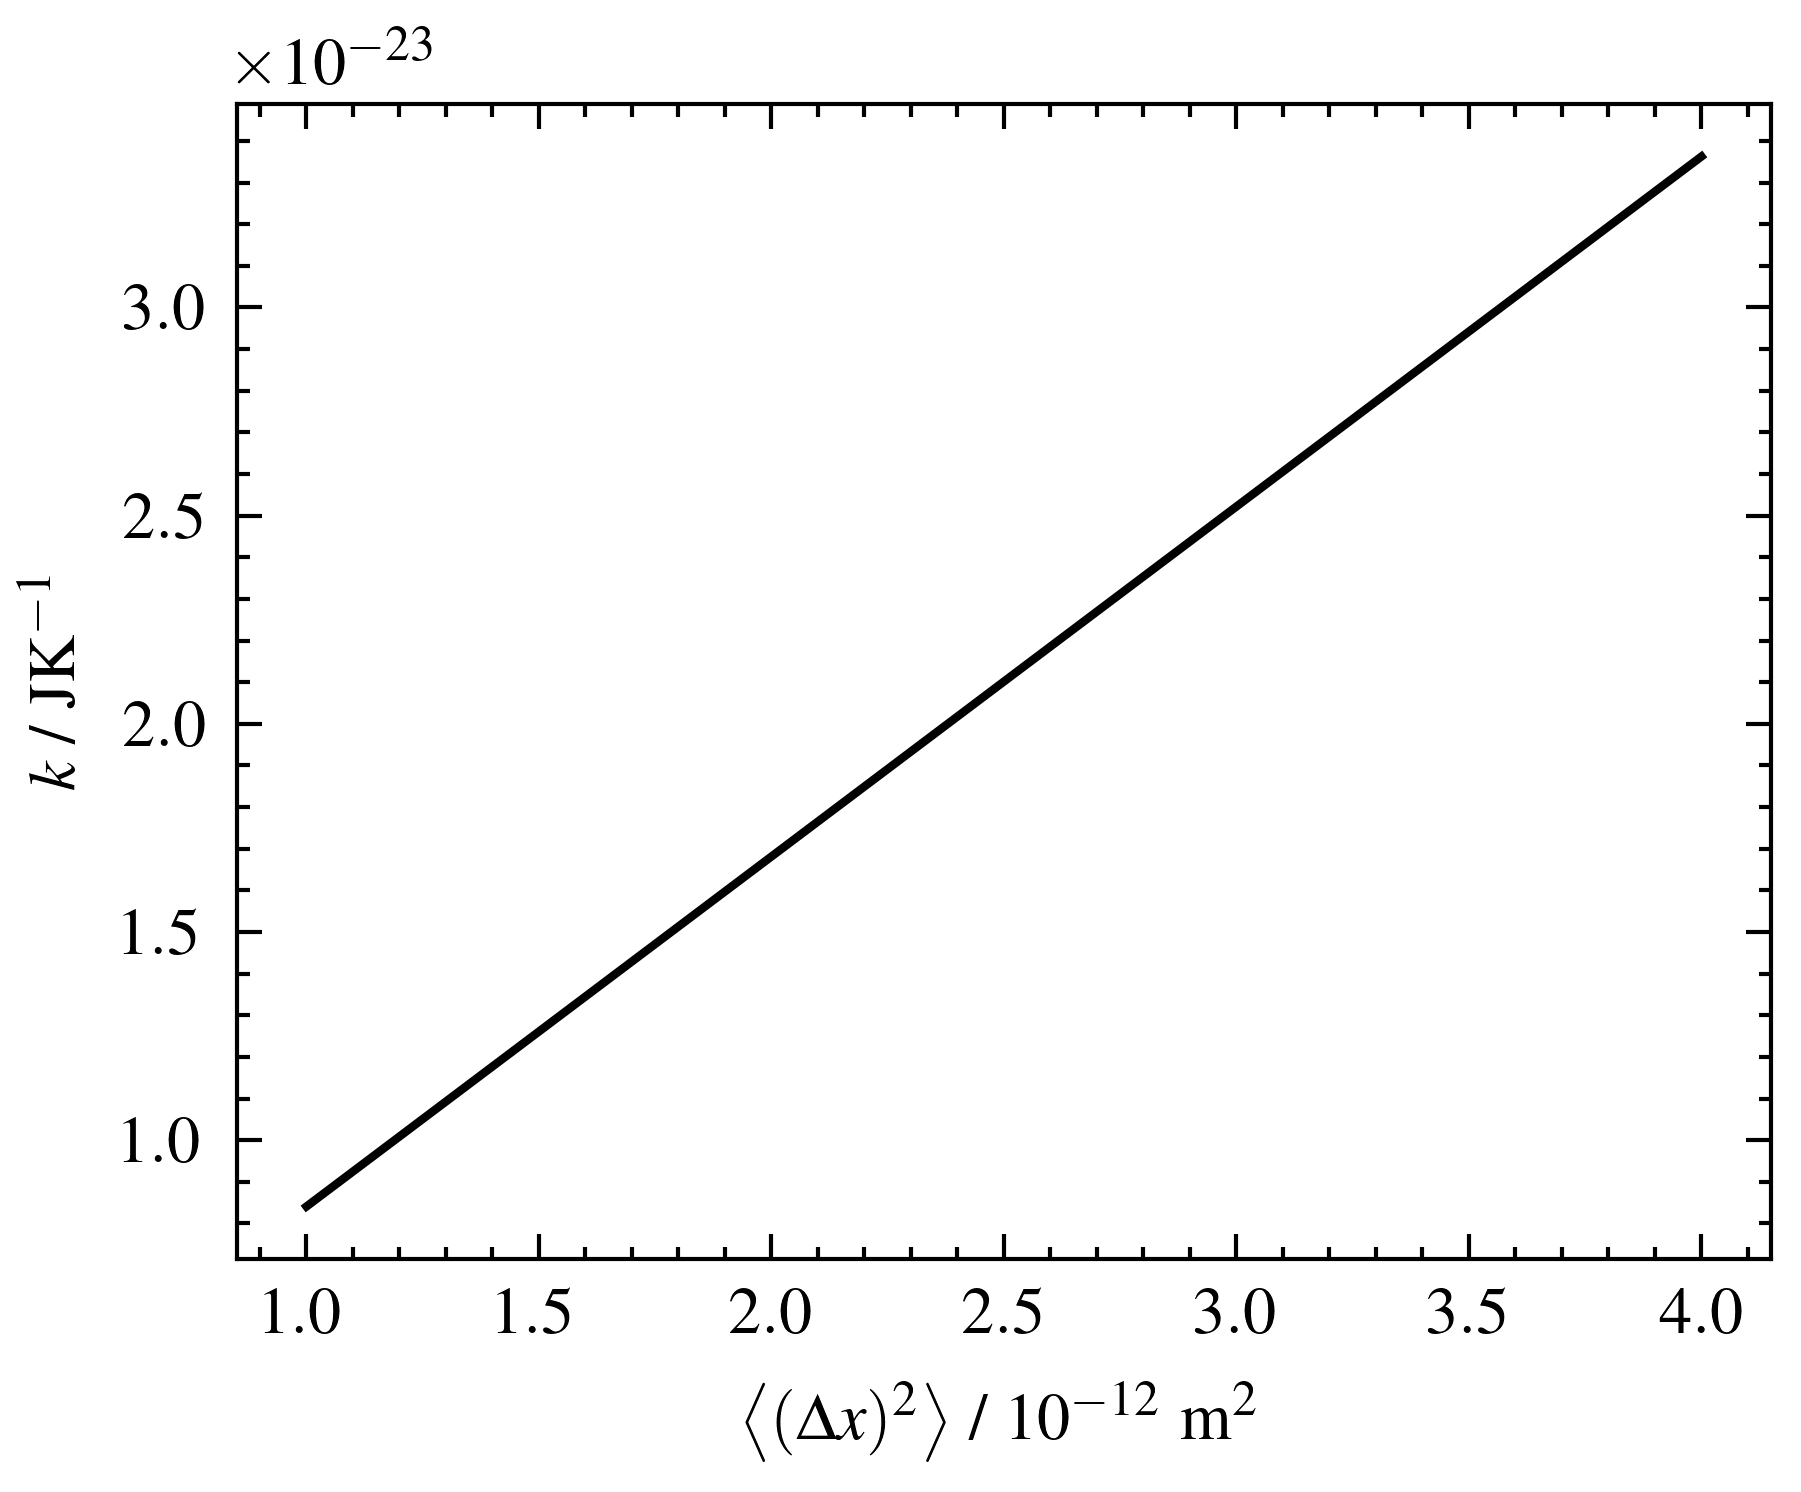
\includegraphics[keepaspectratio, width=0.8\linewidth]{src/figures/k-x-relation/k-x-relation.png}
    \caption{$k$と位置の移動量の分散$\ev{(\Delta x)^2}$の関係}\label{fig:k-x-relation}
\end{figure}


\clearpage
\subsection{課題4}
ブラウン運動を起こすのは水分子の運動による、微粒子との衝突である。
そこで、水分子の速度を考える。

まず気体分子運動論的に考えると、
水分子の運動エネルギー$\dfrac{1}{2}m\bm{x}^2$は、
熱エネルギー$\dfrac{3}{2}kT$と等しいから、
\begin{align}
    \dfrac{1}{2}m\bm{x}^2 & = \dfrac{3}{2}kT \nonumber \\
    \bm{x}^2              & = 3kT/m \nonumber
\end{align}
水分子はランダムに等方的に運動すると仮定すると、
$\bm{x}^2 = {v_x}^2 + {v_y}^2 + {v_z}^2$であるから、
${v_x}^2 = {v_y}^2 = {v_z}^2 = kT/m$である。
よって水分子の速度を$v$とすると、
\begin{align}
    v       & = \sqrt{\dfrac{kT}{m}} \nonumber                                                                                                                  \\
    v_{k_x} & = \sqrt{\dfrac{\SI{3.10E-23}{\joule\per\kelvin} \times \SI{299.35}{\kelvin}}{\SI{18E-3}{\kilo\gram\per\mol} / \SI{2.68E23}{\per\mole}}} \nonumber \\
            & = \SI{372}{\meter\per\second}                                                                                                                     \\
    v_{k_y} & = \SI{372}{\meter\per\second}
\end{align}
と計算できる。

統計力学的に考えると、水分子の速度はMaxwell-Boltzmann分布に従う。
その確率密度関数$f(v)$は、
\begin{equation}\label{eq:maxwell-boltzmann-distribution}
    f(v) = \sqrt{\dfrac{2}{\pi}} \left(\dfrac{m}{kT}\right)^{3/2} v^2 \exp\left(-\dfrac{mv^2}{2kT}\right)
\end{equation}
で与えられる。
\begin{figure}
    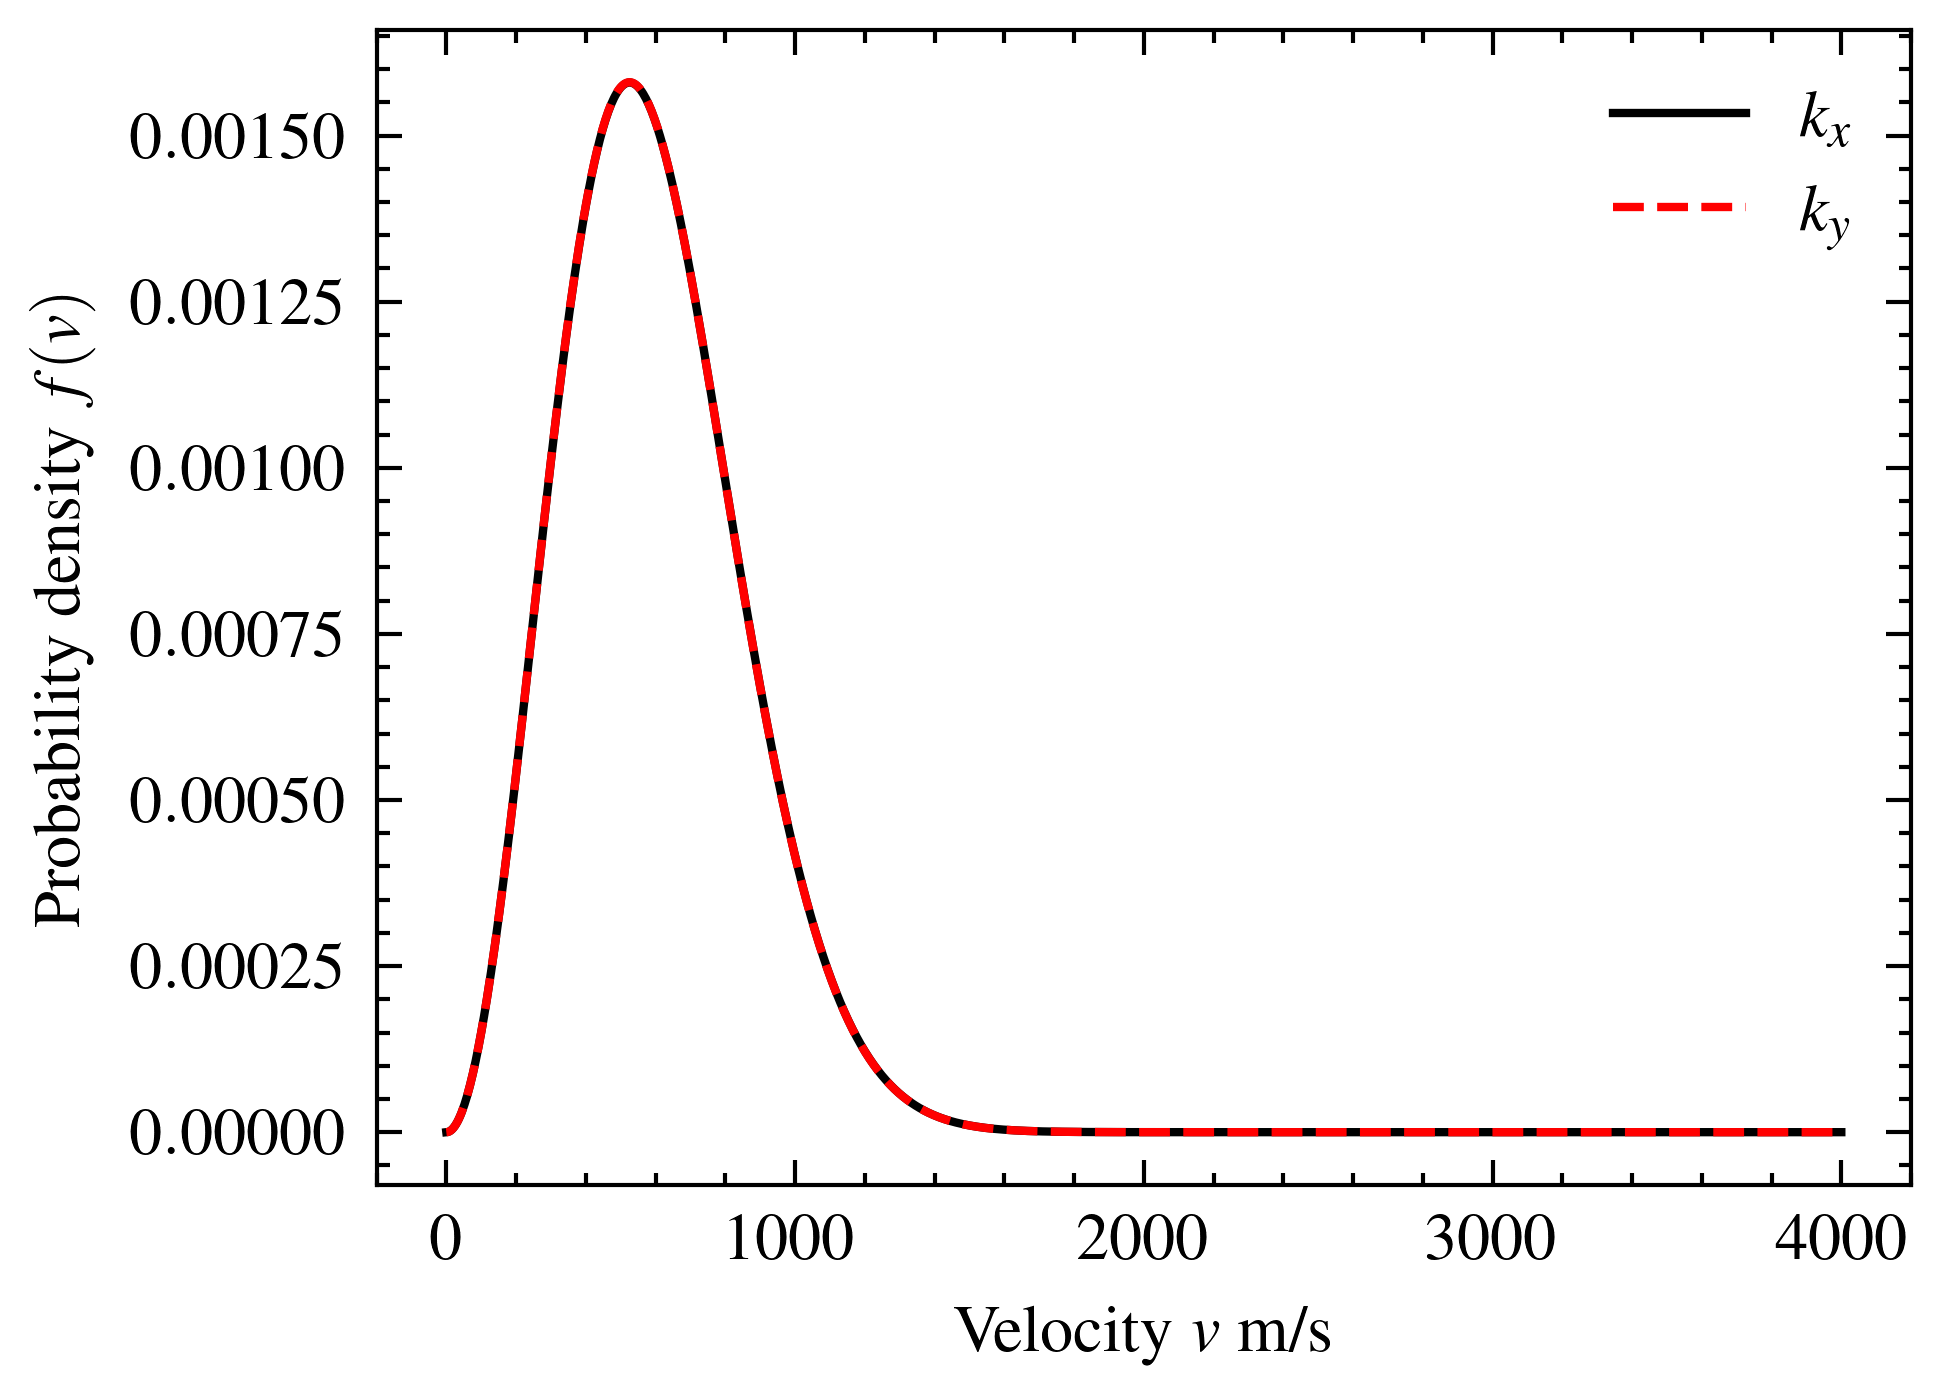
\includegraphics[keepaspectratio, width=0.8\linewidth]{src/figures/maxwell-boltzmann-distribution/maxwell-boltzmann-distribution.png}
    \caption{Maxwell-Boltzmann分布}\label{fig:maxwell-boltzmann-distribution}
\end{figure}

ここで、$m$は水分子の質量、$k$はボルツマン定数、$T$は温度である。
$f(v)$の平均速度$\ev{v}$、二乗平均$\ev{v^2}$は、
\begin{align*}
    \ev{v}   & = \int_0^\infty vf(v)dv                                                                                               \\
             & = \int_{0}^{\infty} \sqrt{\dfrac{2}{\pi}} \left(\dfrac{m}{kT}\right)^{3/2} v^3 \exp\left(-\dfrac{mv^2}{2kT}\right) dv \\
             & = \sqrt{\dfrac{8kT}{\pi m}}                                                                                           \\
    \ev{v^2} & = \int_0^\infty v^2f(v)dv                                                                                             \\
             & = \dfrac{3kT}{m}
\end{align*}
となり、気体分子運動論における式$mv^2/2 = kT/2$の$v^2$は$\ev{v^2}$に等しいことがわかる。

$v$の分散$\ev{(v - \ev{v})^2}=\ev{v^2}-\ev{v}^2$は、
\begin{equation}
    \ev{(v - \ev{v})^2} = \dfrac{(3\pi - 8)kT}{\pi m}
\end{equation}

\clearpage

\subsection{課題5}
分子が存在しないと仮定し、
ランダムに微粒子が動く理由を考える。

微粒子が微小な電荷をもち、水にも微小でみたときに部分的にランダムに電荷があるとすると、
微粒子は水の部分的な電荷の偏りによって斥力や引力がランダムに働き、
その結果としてランダムに動くと仮説を考える。

この仮説を検証するためには、まず水が微小でみたときに部分的にランダムな電荷があるか、
それを持つことが可能か、を検証する必要がある。
定性的に考えると、
ランダムな電荷が存在すればその方向へと移動しランダムな電荷は消失するように考えられるが、
水の粘性によって移動が妨げられるとすればある程度の電荷が存在することが可能であると考えられる。
検証するためには、流体力学的考察と\si{\micro\meter}オーダーの水滴に対して
電場を加え移動するかという実験を行うことが考えられる。
そして、電荷があるとしたら、電磁気学的・古典力学的な理論で
微粒子がランダムに動くことがあるかを説明できるかを検証する必要がある。


\clearpage
\subsection{課題6}

\subsubsection{}
マイクロメーターの1メモリの長さを測るのではなく、できる限り長く測る
なぜならば、1メモリの長さをはかろうとすると、測定誤差がそのまま
1メモリの誤差となる。
例えば、実際の値が\SI{10}{\micro\meter}で測定値が\SI{10.01}{\micro\meter}であるとすると、
誤差は\SI{0.01}{\micro\meter}である。
しかし、できる限り長いメモリ分を計測すればその分割ることができ誤差は小さくなる。
6メモリ分計測し、実際の値が\SI{60}{\micro\meter}で測定値が\SI{60.01}{\micro\meter}であるとする、
誤差は$\SI{0.01}{\micro\meter} / 6 = \SI{0.0017}{\micro\meter}$となる。

\subsubsection{}
マイクロメータの線と垂直に計測できるようなソフトウェアを使用する。
マイクロメータの線に対してソフトウェア上では直線を引き計測したが、
この直線とマイクロメータのなす角が\SI{90}{\degree}からずれていれば、誤差が生じる。
例えば、$\Delta \theta$だけずれていたとすると、実施の値を$l_r$、測定値を$l_m$とすると、
\begin{align*}
    l_r & = l_m \cos \Delta \theta
\end{align*}
となる。
$\Delta \theta=\SI{1}{\degree}$で$\cos\Delta\theta = 0.9998477$であるから、
誤差はそこまで大きくなるわけではないが、
できるだけ正確に測定するためには、マイクロメータの線と垂直に計測することが望ましい。

\clearpage
\subsection{課題7}

\subsubsection{熱雑音}
熱雑音とは、抵抗体内の電子の熱運動によって生じる雑音のことである。
1927年に発見され、ジョンソン-ナイキスト・ノイズとも呼ばれる。
熱雑音の電圧$V_n$は、
\begin{align*}
    V_n = \sqrt{4kTBR}
\end{align*}
と表される。
ここで、$k$はボルツマン定数、$T$は温度、$B$は帯域幅、$R$は抵抗値である。
一般に理想的な帯域幅を持つことはないため、熱雑音の計算は簡単ではないが、
熱雑音の振幅はガウス分布に従い、その振幅スペクトルは平坦な白色雑音である。

\clearpage
\subsection{課題8}
ブラウン運動をコンピュータでシミュレーションしてみる。
\begin{equation}\label{eq:brownian-motion-diff-eq}
    m \odv{\bm{v}}{t} = -\alpha \bm{v} + \bm{f}
\end{equation}
これをコンピュータで解くために差分方程式化すると、
\begin{align}\label{eq:brownian-motion-diff-eq-diff}
    m \dfrac{\bm{v}_{i+1} - \bm{v}_i}{\Delta t} & = -\alpha \bm{v}_i + \bm{f} \nonumber                                                 \\
    \bm{v}_{i+1}                                & = \left( 1 - \dfrac{\alpha \Delta t}{m} \right) \bm{v}_i + \dfrac{\bm{f} \Delta t}{m}
\end{align}
となる。
よって、
\begin{align}\label{eq:brownian-motion-diff-eq-diff-sum}
    \bm{v}_{i} & = \left(1 - \dfrac{\alpha \Delta t}{m}\right)^n \bm{v}_0 + \dfrac{\Delta t}{m} \sum_{i=0}^{n-1} \left(1 - \dfrac{\alpha \Delta t}{m}\right)^i \bm{f}_i
\end{align}
となる。

今、簡単のために$x$のみを考え、粒子の平均速度は0が期待されるから、$\ev{v} = 0$で
$\ev{(v - \ev{v})^2} = \ev{v^2}$である。
多くの粒子についての分散として、$\ev{(v - \ev{v})} = \ev{v^2} - \ev{v}^2$を計算すると、
\begin{align*}
    \ev{v^2} = \left(1 - \dfrac{\alpha \Delta t}{m}\right)^{2n} \ev{(v_0 - \ev{v_0})^2} + \left(\dfrac{\Delta t}{m}\right)^2 \sum_{i=0}^{n-1} \left(1 - \dfrac{\alpha \Delta t}{m}\right)^{2i} \ev{(f_i - \ev{f_i})^2}
\end{align*}
$\ev{(f_i - \ev{f_i})^2}$は、$f$が同一の確率分布に従うとき、
$\ev{(f_i - \ev{f_i})^2} = \ev{(f - \ev{f})^2}$として、
\begin{align*}
    \ev{v^2} & = \left(1 - \dfrac{\alpha \Delta t}{m}\right)^{2n} \ev{(v_0 - \ev{v_0})^2} + \left(\dfrac{\Delta t}{m}\right)^2 \ev{(f - \ev{f})^2} \sum_{i=0}^{n-1} \left(1 - \dfrac{\alpha \Delta t}{m}\right)^{2i} \nonumber                                         \\
             & = \left(1 - \dfrac{\alpha \Delta t}{m}\right)^{2n} \ev{(v_0 - \ev{v_0})^2} + \left(\dfrac{\Delta t}{m}\right)^2 \ev{(f - \ev{f})^2} \dfrac{1 - \left(1 - \dfrac{\alpha \Delta t}{m}\right)^{2(n-1)}}{1 - \left(1 - \dfrac{\alpha \Delta t}{m}\right)^2}
\end{align*}
ここで、$\Delta t$を十分小さくとり、$n \to \infty$とすると、
\begin{align}
    \ev{v^2} & = \left(\dfrac{\Delta t}{m}\right)^2 \ev{(f - \ev{f})^2} \dfrac{1}{1 - \left(1 - \dfrac{\alpha \Delta t}{m}\right)^2} \nonumber \\
             & \approx \dfrac{\Delta t}{2 \alpha m} \ev{(f - \ev{f})^2}
\end{align}
を得る。
気体分子運動論から、$\ev{v^2} = kT/m$であるから、
\begin{equation}
    \ev{(f - \ev{f})^2} = \dfrac{2 \alpha kT}{\Delta t}
\end{equation}
よって、この分散をもつ正規分布に従う乱数を生成し、
\begin{equation}
    x_n = x_{n-1} + v_{n-1} \Delta t
\end{equation}
で位置を計算すればよい。

このシミュレーションを行った結果を図\ref{fig:brownian-2d-sim}に示す。
\begin{figure}
    \centering
    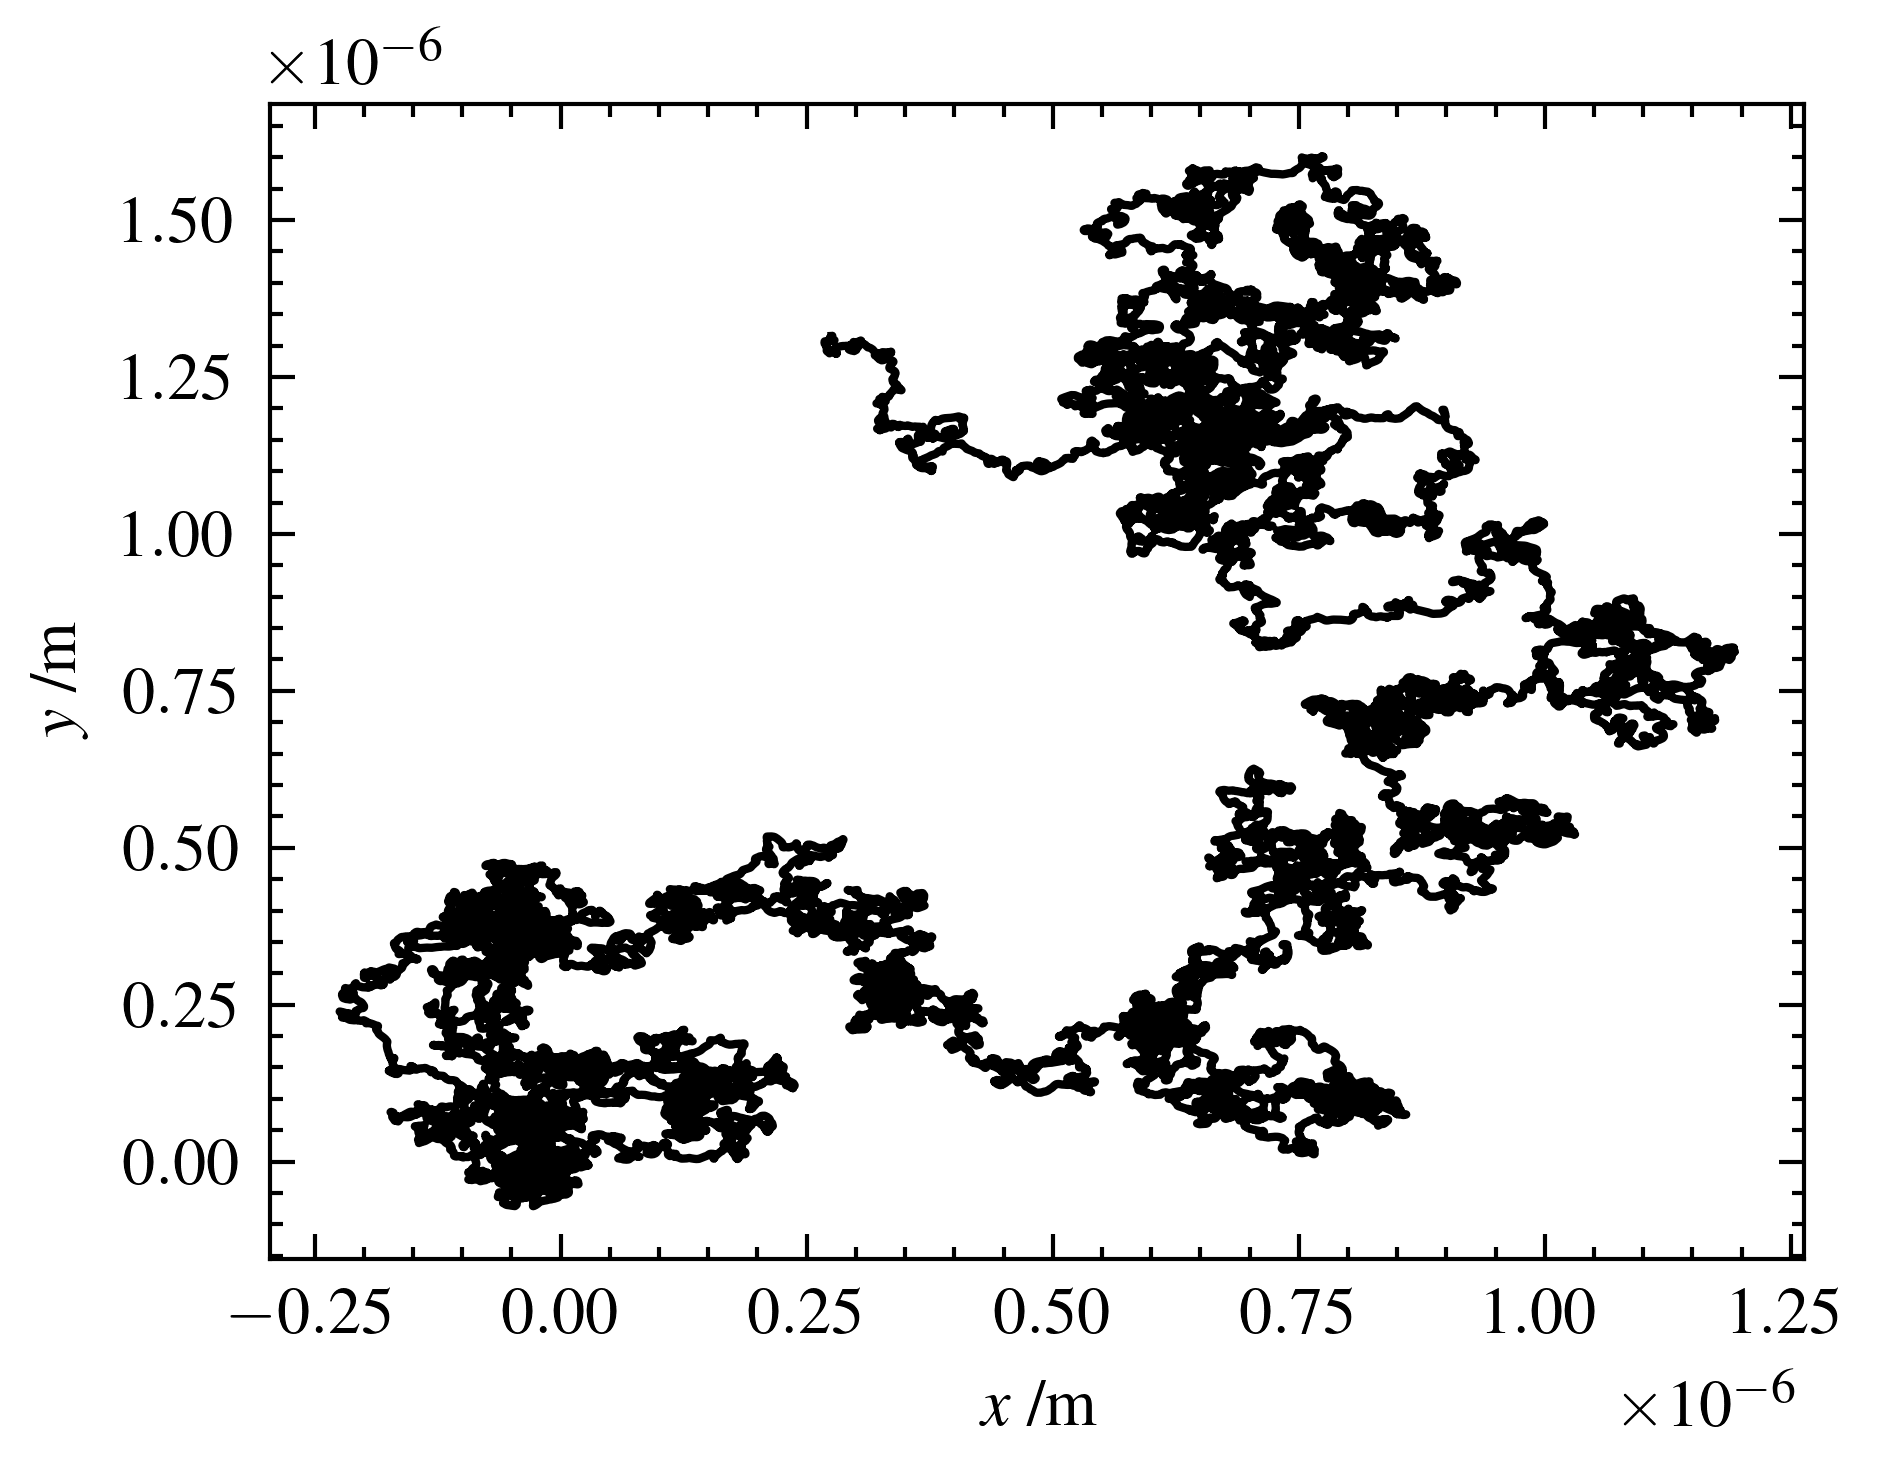
\includegraphics[width=0.8\linewidth]{./src/figures/brownian-2d-sim/brownian-2d-sim.png}
    \caption{2次元ブラウン運動のシミュレーション}\label{fig:brownian-2d-sim}
\end{figure}

この図を見ると、光学顕微鏡で見れる\si{\micro\meter}のオーダーで、
ランダムに動く粒子の動きが再現できている。






\end{document}
